\documentclass{article}
\usepackage[utf8]{inputenc}
\usepackage{amsfonts}
\usepackage{amsmath}
\usepackage{amssymb,amsmath,color}
\usepackage{graphicx}
\usepackage{float}
\usepackage{afterpage}
\usepackage[pdfencoding=auto]{hyperref}
\usepackage{bookmark}% faster updated bookmarks
\usepackage{todonotes} %\todo{}
\usepackage{comment}
\usepackage{natbib}
\usepackage{mathtools}
\usepackage{stackengine}
\usepackage[bb=boondox]{mathalfa}
\usepackage{hyperref}
%%fonts declaration

%%
%%symbols declaration 
\DeclareMathAlphabet\mathbfcal{OMS}{cmsy}{b}{n} %for calligraphy letters
\DeclareMathOperator*{\argmin}{argmin}
\DeclarePairedDelimiter{\norm}{\lVert}{\rVert} 
%end symbol declaration
\def\blankpage{%
      \clearpage%
      \thispagestyle{empty}%
      \addtocounter{page}{-1}%
      \null%
      \clearpage}
\def\delequal{\mathrel{\ensurestackMath{\stackon[1pt]{=}{\scriptstyle\Delta}}}}
\graphicspath{ {./images/} }
\begin{document}
%%%%%%%%%%% Cover %%%%%%%%%%%
\thispagestyle{empty}                                                 
\begin{center}                                                            
    \vspace{5mm}
    {\LARGE UNIVERSIT\`A DI BOLOGNA} \\                       
      \vspace{5mm}
\end{center}

\begin{center}
  
\includegraphics[scale=.27]{images/logo_unibo.png}
\end{center}

\begin{center}
      \vspace{5mm}
      {\LARGE School of Engineering} \\
        \vspace{3mm}
      {\Large Master Degree in Automation Engineering} \\
      \vspace{20mm}
      {\LARGE Distributed Control Systems} \\
      \vspace{5mm}
      {\Large\textbf{Course Project 3}}\\
      {\Large\textbf{Distributed Task Assignement for Robotic Network}}
      \vspace{15mm}
\end{center}

\begin{flushleft}                                                                              
     {\large Professor: \textbf{\@ Giuseppe Notarstefano}} \\  
     {\large Tutor: \textbf{\@ Andrea Testa}} \\
      \vspace{13mm}
\end{flushleft}
\begin{flushright}
      {\large  {GROUP 22}}\\
      {\large \underline {Students:}}\\
      {\large Francesco Cerri}\\
      {\large Gianmarco Canello}\\
      {\large Marco Roncato}\\
\end{flushright}        %capoverso allineato a destra
\begin{center}
\vfill
      {\large Academic year \@2020/2021} \\
\end{center}

%%%%%%%%%%%  end Cover %%%%%%%%%%%

\blankpage{}

%%%%%%%%%%%  Chapter list%%%%%%%%%%%

\begin{center}

\thispagestyle{empty}
\Large\tableofcontents \thispagestyle{empty}
\newpage
\listoffigures\thispagestyle{empty} 

\end{center}



%%%%%%%%%%%  end Chapter list %%%%%%%%%%%

\newpage

%%%%%%%%%%%  chapter 1 %%%%%%%%%%%
\section{Introduction}
\subsection{Problem introduction}
The aim is to model and control of a network of robots that need to
self-assign a set of tasks in target locations by running an optimization algorithm. The objective of this algorithm is to choose an assignment that optimizes the total path length between tasks and robots. The optimization problem can be approached in a centralized fashion or in a distributed way.
A centralized optimization algorithm works using the definitions of hive and drones, where the drones send to the hive the gathered information to be computed and the hive performs computations and replies to the drones with the orders to be followed. In a distributed algorithm there is no hive and drones communication,instead we rely on agents that communicate among each other in order to decide the best action to perform.
The problem is well posed and admits a solution in both the approaches, although the uniqueness and the quality of the solution may vary depending on the domain in which the optimization problem is evaluated.

\subsection{Tools used}
\begin{comment}
\end{comment}
In order to solve the optimization problem we wrote program \citep{Omni} have used basic MATLAB functionalities and the Optimization toolboxes. Regarding the theoretical part, we have used the knowledge of cost coupled optimization principles presented in the Bullo's book \citep{Bullo} and in the paper by Testa & Notarstefano \citep{Testa} ; various tries were carried out by doing a Montecarlo simulation for the resolution of the general linear problem, with varying agent number and dimension, and for the particular case of assignation,with the agent and task positions randomized inside an interval decided by the user. The spawn area of the agents and tasks is a square. 


\subsection{Motivations}
Solving the Generalized Assignment Problem (GAP) is detailed in \citep{Testa} and \citep{Nostro}  and they provide us a solution that could be implemented in any application in which is required to assign tasks to agents with a predefined criteria (e.g. path length, agents capability to solve that task, ecc).
Even though the GAP problem is a NP-hard problem, and there are several solution in optimization literature, we are trying to provide a robust solution able to cope possible noise that could interfere inside robot communication


\subsection{Applications}
This type of algorithm is needed in various fields: robotics, for example the optimization of the route for robots that carry items inside a warehouse or a factory, logistics, for example maximizing fuel efficiency of delivery trucks. In general, this algorithm is used when we want to minimize the energy used to complete a certain task made by a large number of independent agents that are able to communicate between themselves.  

\subsection{Contributions}
We have developed some MATLAB simulations in order to show the algorithm working.
As a first effort, we have written a problem generator file that can be configured to perform the generation of matrices for both of the assigned tasks: in the first task the problem generation can be personalized by giving the dimension of the  the number of agents and the number of tasks, conversely in the second task we can also add the width and height of the spawn area, presence of noise in the computation of the cost and also the "noRestrictions" parameter defining the capability of all the agents to perform any task(in the normal execution not all the agents can perform every task).
In the first task we simulated the convergence error of agents and tasks under polyhedron constraints by defining a domain in which the agents could spawn and then be compared to a centralized algorithm solution of the same problem.
In the second task we simulated an application of the first task via the graphical representation of agents that need to decide, in distributed fashion, which task to perform among them to minimize the total travelled distance . 

%%%%%%%%%%% end chapter 1 %%%%%%%%%%%

\section{Constrained coupled linear problems} 
The task assignment problem can be formulated as this particular class of linear problems; in this chapter, we'll present a brief introduction to the theory that allows us solve the said problem. Given a cost function, separable with respect to agents, each of them defined in a particular subset, and a set of equality constraints, the problem can be formulated as 

\begin{align}
  &\min_{x_i\in X_i} \sum_{i=1}^{N} f_i(x_i) \\
  &\text{subj.to} \   h_l(x)-b_l=0 \ &\quad \forall l \in {1,\dots, m} \\
  & x_i\in X_i \subset \mathbb R^{n_i} , &\quad \forall i \in {1,\dots, N}
\end{align}
with ${f_i:\mathbb R^{n_i} \rightarrow \mathbb R }$ convex, ${h_l:\mathbb R^{n_i} \rightarrow \mathbb R}$ convex and ${X_i \subset \mathbb R^{n_i}}$ convex and compact.\\
\\
In the cases in which the gradient of the cost function cannot be calculated, it is possible to use the subgradient method: this algorithm can be implemented in a distributed fashion to solve the constrained coupled optimization problem.


\subsection{Distributed Dual Subgradient algorithm}
We can solve the constrained coupled optimization problem via the dual distributed subgradient algorithm 
\begin{align}
    v_i^{t+1} &= \sum_{j\in \mathcal{N}_i}^{} a_{ij}\lambda_j^t \\
    x_i^{t+1} &=  \argmin_{x_i\in \mathcal{X}_i} f_i(x_i) + (v_i^{t+1})^Th_i(x_i)\\
    \lambda_i^{t+1}&=v_i^{t+1}+\alpha^th_i(x_i^{t+1})
\end{align}

\noindent the optimal solution for the dual problem is given by maximizing ${q(\lambda)}$ 
with 
\begin{equation} q(\lambda)= \inf_{x\in P} L(x,\lambda) \end{equation} 
\begin{equation}   L(z,\lambda) = \sum_{i=0}^{N} f_i(x_i) + \sum_{l=0}^{S}\lambda_l(\sum_{i=1}^{N}H_i x_i-b_l) \quad b \in {\mathbb R}^S 
\end{equation}

\noindent In general we know for sure that weak duality always holds (e.g. ${q^*\leq f^*}$) ,
thus
\begin{equation}
    q^*=\sup_{\lambda} \leq \inf_{x \in \mathbb{X}}=f^*
\end{equation}

Therefore by maximizing the dual function we can define a lower bound for the optimal cost of the primal problem, Although we need strong duality in order to nullify the duality gap (e.g. ${q^*\leq f^*}$). \\
in order to get the Strong duality we need to have a "Convex Problem":
\begin{enumerate}
    \item ${ X\subset {\mathbb R}^d}$ convex;
    \item ${f}$ finite and convex over X;
    \item ${h_l}$ are affines;
    \item  ${\exists \ \overline{x} \in ri(X)}$ s.t. ${h_l(\overline{x})-b=0}$ ;
    
\end{enumerate}
if the previous assumption hold for the primal problem. Then there is no duality gap, i.e., ${q^* = f^*}$ .
This does not solve our main problem of evaluating the optimal value for the decision valuables ${x}$, we need to make some extra evaluation in order to obtain the optimal values of the decision variables by making the 
  
  \begin{align}
  & \min_{x \in X} \ f(x) \\
  &\text{subj.to}  \ h_l(x)-b=0 \quad l\in {1,\dots, m}  \\
\end{align}
  
\noindent Assuming that

\begin{enumerate}

\item ${a_{ij}\ i,j\in{1,\dots, N}}$ be non negative entries of a weighted adjacency A to the undirected graph ${\mathcal{G}}$, with ${a_{ij}>0}$ and ${A}$ doubly stochastic;
\item the step-size sequence ${\{\alpha^{t}\}_{t\geq 0}}$, satiesies the conditions

\begin{align}
    \alpha^{t}\geq0,\ \sum_{t=0}^{\infty} \alpha^{t}=\infty,\ \sum_{t=0}^{\infty} (\alpha^{t})^2<\infty
\end{align}

\item ${\forall i \in {1,\dots, N}}$  : each function ${f_i}$ is convex, each constraint ${\mathcal{X}_i}$ is non-empty, compact and convex set; each function ${h_i}$ is a component-wise convex function. \\Moreover, there exist ${\overline{x}_1\in X_1,\dots,\overline{x}_N\in X_N}$ such that${\sum_{i=1}^{N} h_i(\overline{x}_i)<0}$ 
\end{enumerate}

\noindent Let assumptions 1, 2 and 3  hold, then the sequence of dual variables ${\lambda_1^t,\dots,\lambda_N^t}$ with ${t\geq0}$ generated by the Distributed Dual Subgradient satisfies:
\begin{align}
    \lim_{t \to \infty}\norm{\lambda_i^t-\lambda^*}=0, \\ i\in\{1,\dots, N\},
\end{align}
where ${\lambda^*}$ is an optimal solution of the dual problem. Moreover, let for each t,
\begin{align}
    \widehat{x_i}^t= \frac{1}{t} \sum_{\tau=0}^{t} x_i^\tau
\end{align}
Then, it holds
\begin{align}
    \lim_{t \to \infty} \sum_{i=1}^{N} f_i(\widehat{x_i}^t) &= f^*,\\
    \lim_{t \to \infty}\norm{\widehat{x_i}^t-x^*}&=0, & i\in\{1,\dots,N\},
\end{align}
where ${x^*}$ and ${f^*}$ denote an optimal solution and the optimal cost of the primal problem. 

\section{Distributed constrained coupled problem }

\subsection {Problem introduction}
In the first task we are considering a constrained coupled linear problem in distributed scenario of a set of ${N}$ agents in ${\mathbb R}^m$ where ${n_i}$ are the number of components in the state vector of the agents and S are the number of equality constraints the optimization problem is subject to. 
The problem can be defined as follow:
\begin{align}
  \min_{z_1,...,z_N} & \sum_{i=1}^{N} c_i^Tz_i \\
  \text{subj.to} &\sum_{i=1}^{N} H_iz_i=b  \\
  & z_i\in P_i , \quad \forall i \in {1,\dots, N}
  & c_i \in {\mathbb R}^{n_i}\\
  & H_i \in {\mathbb R}^{S\times n_i} 
  & b\in {\mathbb R}^S
\end{align}

\noindent With $P_i$ being the compact polyhedron described by linear equality and inequality constraints; in practical sense, this polyhedron can be seen as a sensor range of the agent.

\begin{align}
    P_i &\delequal \{z_i \in {\mathbb R}^n_i | D_i z_i \leq d_i, G_i z_i = g_i\} & \forall i \in \{1\dots N\}
\end{align}

\noindent Lagrangian equation of the task

\begin{align}
    L(z,\lambda) &= \sum_{i=0}^{N} c_i^T z_i + \sum_{l=0}^{S}\lambda_l(\sum_{i=1}^{N}H_i z_i-b_l) & b \in {\mathbb R}^S
\end{align}
The dual function then is:
\begin{align}
    q(\lambda) &= \inf_{z\in P}L(z,\lambda) = \inf_{z\in P} \sum_{i=0}^{N} c_i^T z_i + \sum_{l=0}^{S}\lambda_l(\sum_{i=1}^{N}H_i z_i-b_l)
\end{align}
Since we are in a distributed scenario the lambda has the following vector form:
\begin{gather}
 \begin{bmatrix} \lambda_1^{t+1} \\ \vdots \\ \lambda_s^{t+1} \end{bmatrix} 
 =
 \begin{bmatrix} v_1^{t+1} \\ \vdots \\ v_s^{t+1} \end{bmatrix} +\alpha^t \begin{bmatrix} \sum_{i=1}^{N}H_i z_i^{t+1}-b_1 \\ \vdots \\ \sum_{i=1}^{N}H_i z_i^{t+1}-b_s \end{bmatrix} 
\end{gather}
 
\noindent Where $v_i^{t+1}$ are the aggregation variables produced by weighting the current neighbours' lambdas as previously shown in (4).
We can evaluate $z_i^{t+1}$ by means of the following relation obtained by (6):
\begin{equation}
    z_i^{t+1} =  \argmin_{ {D_iz_i \leq d_i} \atop 0\leq z_i\leq 1;  } (c_i + v_i^{t+1}H_i)z_i
\end{equation}

therefore by applying the results of (16),(17)and(18) we are able to find the optimal value for the decisions variables

\subsection {Assumptions for the execution}
In order to solve the problem some assumption should be made in order to set the problem and then test it inside MATLAB environment:
\begin{itemize}
    \item The values of $c_i$ are randomly generated in order to give different weights to agents inside the optimization problem;
    \item The dimension of the state vector of the agents coincides with the dimension of the number of equality constraints active on the optimization problem (e.g $n_i\equiv S$), this assumption is made for the sake of simplicity of producing M equality constraints, but it can be easily generalized to $S \geq M $;
    \item $H_i=\mathbb{1}$ and and $b=[1\dots 1]$ since for the sake of the implementation we want to have the following equality to be satisfied 
    \begin{equation*}
    \sum_{i=1}^{N} z_{ij}=1 \qquad \forall j \in \{1\dots M\}
    \end{equation*}
    this is made order to cap the sum of the k-th state component of all the vector in prevision of the requests inside Optimal task assignment chapter;
    \item $D_i$ and $d_i$ are default chosen in order to impose reasonable shape of the polyhedron,instead $G_i$ and $g_i$ are considered to be null, since for sake of simplicity only equality constraints are take in considerations, consequently the polyhedron becomes:
\begin{equation*}
     P_i = \{z_i \in {\mathbb R}^{n_i} \ | \ D_i z_i \leq d_i\} \qquad \forall i \in \{1\dots N\}
\end{equation*}
   \item the UB and LB are respectively chosen to make the state components of the agents stay inside the interval $z_{ij}\in \{0,1\}$; 
\end{itemize}


\noindent In the deployed code we generate the above matrices by means of the function progen(), which produces the said matrices by means of the number of agents N and the number of state components of the agents M. Therefore the problem is considered to be defined and can be solved by means of the linear program theory recalled at the beginning of the chapter.\\
Inside the MATLAB project we made use of the function linprog() in order to solve the minimization problem exposed in equation (27) and then, applying the dual sub gradient results, we are able to finally solve our constrained  coupled  linear  problem obtaining the optimal values of the decision variables for each agent.

\subsection {Simulation and results of Monte Carlo experiments for Task 1}
A series of Monte Carlo trials have been performed to extract meaningful statistical indicators for the presented algorithm. While the code permitted to also vary graph characteristics, only the number of agents and their dimension (expressed in term of minimal and maximal "surplus" with respect to agent dimension) were varied.
The implemented code simply re-runned the single trial one previously tested and exported data in form of workspace variables and plots for cost and consensus error.

Each experiment (i.e. an experiment with constant characteristics) is repeated a constant amount of times; the results obtained are then fed to a scripts that averages them, on the total number of repetitions for each experiment. Results of this procedure are provided in form of plots of running average cost  relative error(with respect to centralized solution cost, computed via the MATLAB linprog() function), of primal and dual costs, and consensus error.\\

%%const N
\begin{figure}[h!]
    \centering
    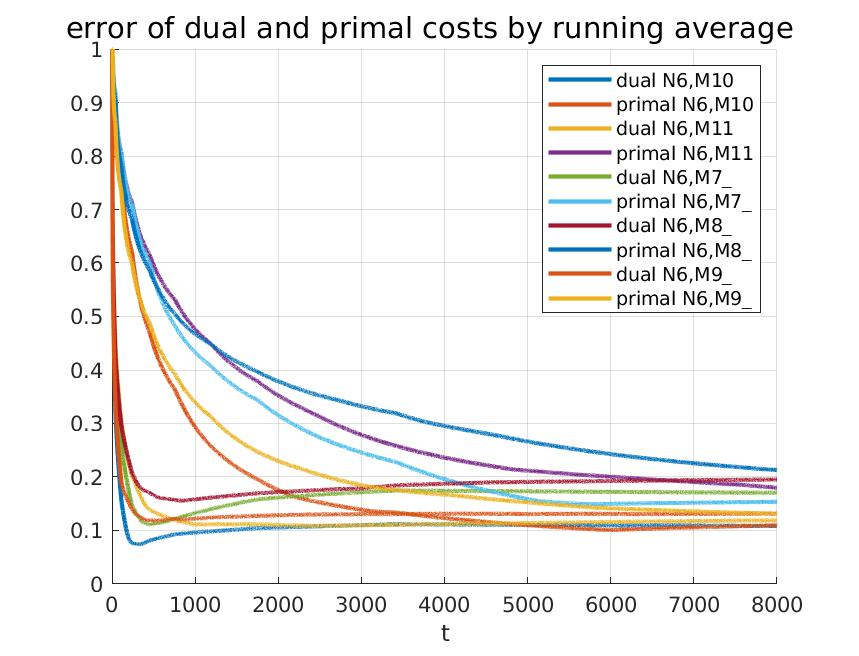
\includegraphics[scale=0.41]{images/aggr_REP10_CostPlot_N6_[M9]_.jpg}
    \caption{running average relative cost error, average on 10 experiments with constant agents number}
    \label{fig:running average cost error plot}
\end{figure}
\begin{figure}[h!]
    \centering
    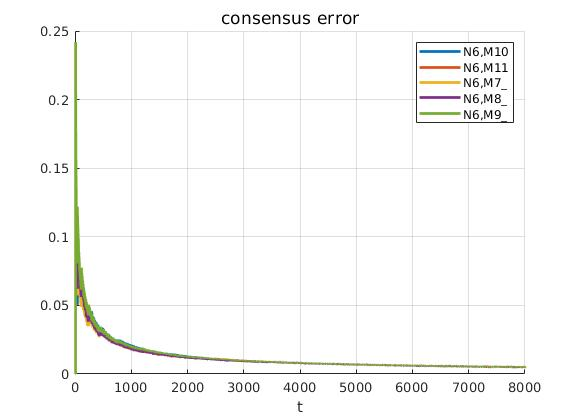
\includegraphics[scale=0.45]{images/aggr_REP10_ConsPlot_N6_[M9]_.jpg}
    \caption{consensus error, average on 10 experiments with constant agents number}
    \label{fig:running average cost error plot}
\end{figure}
\newpage
%%const M
\begin{figure}[h!]
    \centering
    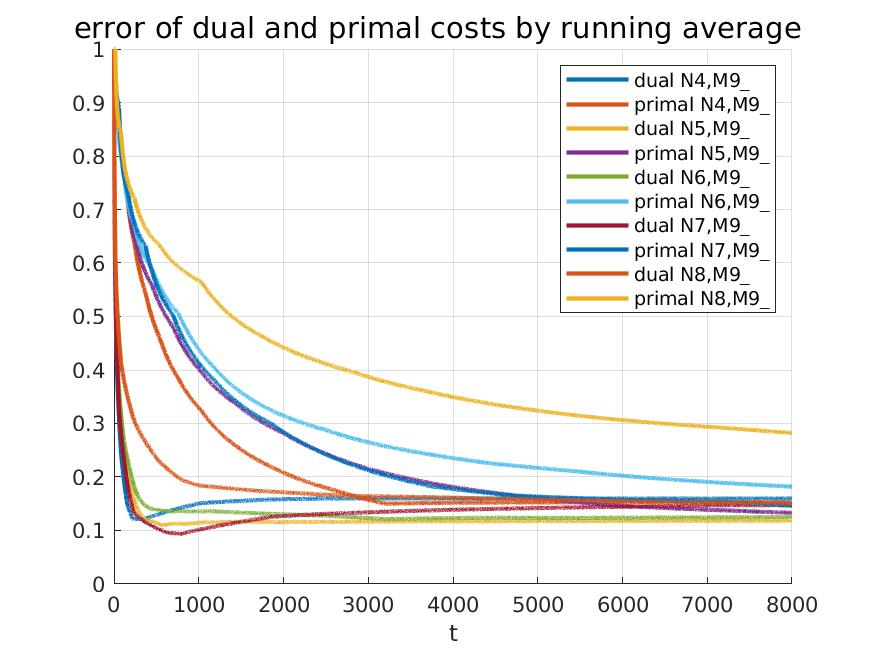
\includegraphics[scale=0.36]{images/aggr_REP10_CostPlot_M9_[N5]_.jpg}
    \caption{running average relative cost error, average on 10 experiments with constant agent dimension}
    \label{fig:running average cost error plot}
\end{figure}
\begin{figure}[h!]
    \centering
    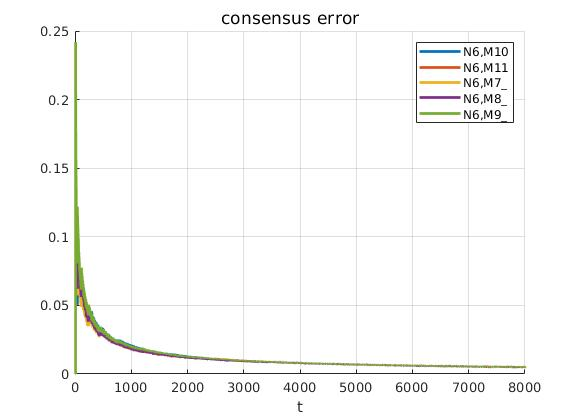
\includegraphics[scale=0.5]{images/aggr_REP10_ConsPlot_N6_[M9]_.jpg}
    \caption{consensus error,  constant agent dimension}
    \label{fig:running average cost error plot}
\end{figure}
\newpage
\newpage
The results of consensus error show a clear and fast convergence for the agents.\\
The results of relative errors consolidates on average at 10 percent, but this is due to the low number of experiment repetitions and the presence of some experiments that worsen the statistics.A more characteristic result for a single, non averaged, experiment are provided to show the capabilities of the algorithm.\\
%%single experiment
\begin{figure}[h!]
    \centering
    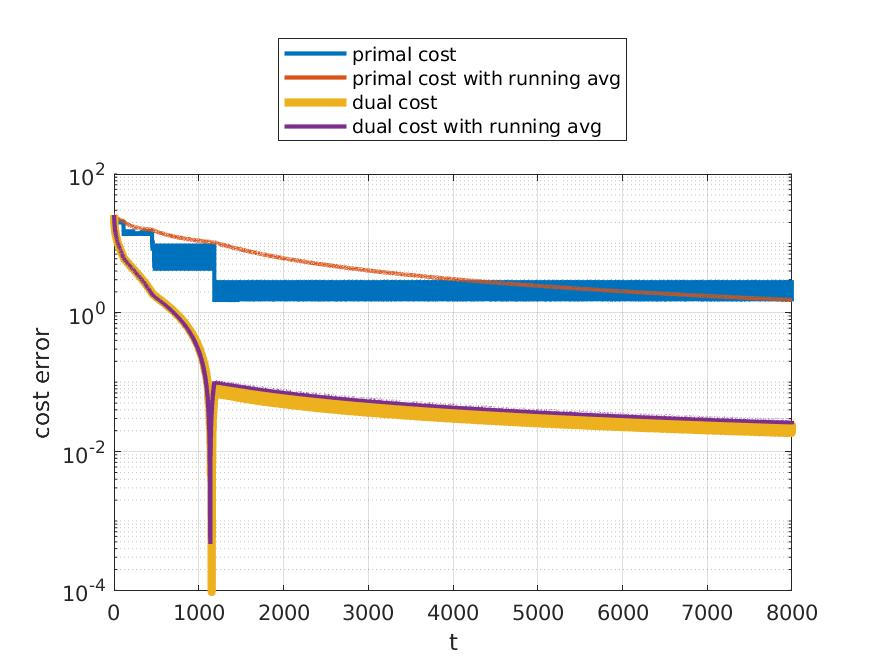
\includegraphics[scale=0.25]{images/N6_M9_STCdoubly_TOPbinomial_PRB1_CostPlot.jpg}
    \caption{running average relative cost error, single experiment}
    \label{fig:consensus error plot}
\end{figure}


\newpage
\section{Optimal task assignment}


\subsection{Problem formulation}
In the task 2 there are N robots trying to self assigning N tasks scattered randomly in the environment each of them must be served by at most one robot, the objective is to minimize the total travelled distance of the agents. To do so we employ the the results achieved in the task 1 in order to use the distributed optimization procedure in order to make the agents self assign the task in a distributed optimization procedure.\\
Define: $V_A$ as the node set, $U_A$ as the task set $E_A$ as the set of edges.
\\
An edge $(i,k) \in E_A$ exists if and only if agent i can be assigned to task k.
The cost $c_{ik}$ (cost of agent i to perform task k) is a weight on the edge, calculated by considering the norm of the distance of agent i to the objective k.
Objective: solve the linear optimization program:
\begin{align}
    \min_{z_1,...,z_N}  &\sum_{i=1}^{N} c_i^Tz_i \\
    \text{subj.to}      &\sum_{k|(i,k)\in E_A} x_{ik} =1 
  & \forall i \in \{1\dots N\}
    \\
   & \sum_{i|(i,k)\in E_A} x_{ik} =1   & \forall i \in \{1\dots N\}
\end{align}
We can reformulate the problem by defining from (citation):(leggi la chat)
\begin{itemize}
\item $z_i$ a vector stacking all $x_{ik} \forall$  k such that (i,k) $\in E_A$
\item $c_i$ a vector stacking all $c_{ik} \forall$  k such that (i,k) $\in E_A$
\end{itemize}
Define the local polyhedron $P_i$ as
\begin{align}
    P_i &\delequal \{x_i \ | \ 0 \leq x_i \leq 1, \sum_{k|(i,k)\in E_A} x_{ik} =1\} & \forall i \in \{1\dots N\}
\end{align}

Also the matrix ${H_i}$ is defined suitably by extracting from the  ${N\times N}$  identity matrix the subset of columns corresponding to the tasks agent i can perform. The b vector is defined as a vector of ones.\\
The problem becomes:\\
\begin{align}
    \min_{z_1,...,z_N} & \sum_{i=1}^{N} c_i^Tz_i \\
    \text{subj.to} & \sum_{k|(i,k)\in E_A} H_iz_i =1 & \forall i \in \{1\dots N\}
    \\
   & with: z_i \in P_i
\end{align}

In our project execution, the matrix $H$ is either created by randomly assigning 0 or 1 to each of the entries or such that every agent can execute any task by activating a toggle inside the code that generates the problem.
\subsection{Problem solution}
The environment where task and robots are spawned is assumed to be a $1\ by 1$ square with dimension 2 (default option, but the code may generate 3d environments too) or possibly a circle with radius 1. Both tasks and robots are spawned randomly inside this space.

%need to explain v, G, LB and UB before this part
To solve the minimization problem, we make use of the linprog function in MATLAB. This function takes as inputs: \\
x = linprog(f,A,b,Aeq,beq,lb,ub,options)\\
with:
\begin{align}
    \min_{x}f^T\ \text{such that} 
    \begin{cases} Ax \leq b\\
        A_{eq} = b_{eq}\\
        lb \leq x \leq ub
    \end{cases}
\end{align}
In this scenario the following choices for the parameters were made:
\begin{align}
    f &= c_i+(v(i,:))*H_i\\
    A_{eq} &= G_i\\
    b_{eq} &= g_i\\
    lb&= LB_i\\
    ub&= UB_i
\end{align}
In the end the primal cost is computed as:
\begin{align}
f_i &= c_i*Z(i,:,t)^T\\
primCost(t)&= primCost(t) + f_i\\     
\end{align}

\
The dual cost is:\\

\begin{align}
  q_i = c_i * Z(i,:,t)^T+\lambda(i,:,t) * ( Z(i,:,t) - b_i^T )^T\\
        dualCost(t) = dualCost(t) + q_i
\end{align}

\newpage

\subsection{Simulation and results of a single experiment for Task Assignment Problem}
Results of converge of the algorithm, applied to the task assignment problem, are stated below.
The plot of cost  clearly show the correctness of the solution, since the curves converges fast to centralized solution value; consensus error curves as well converge fast for all the agents.

\begin{figure}[h!]
\caption{assignment from distributed algorithm}
\centering
 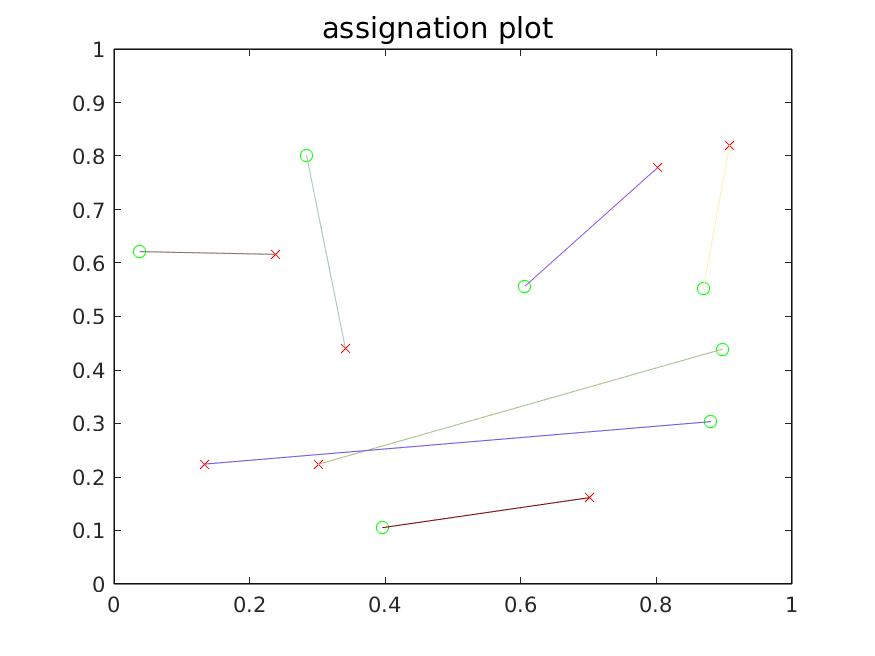
\includegraphics[scale=.38]{images/assign_N7seed_[0_0]_rep2_assiPlot.jpg}

\label{fig: assignment plot}
\end{figure}

\begin{figure}[h!]
\caption{dual (distributed) and centralized costs for assignment}
\centering
 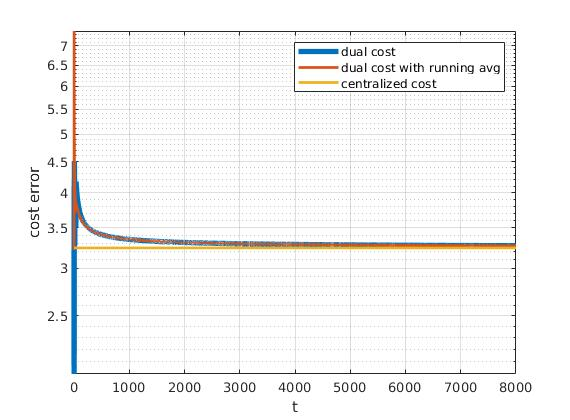
\includegraphics[scale=.58]{images/assign_N7seed_[0_0]_rep2_Cost.jpg}
\label{fig: cost plot}
\end{figure}

In this particular case, the cost calculated by the centralized algorithm is 3.2383, the same exact cost calculated by our algorithm with distributed assignation.


\begin{figure}[h!]
\centering
\caption{consensus error of a single agent}
 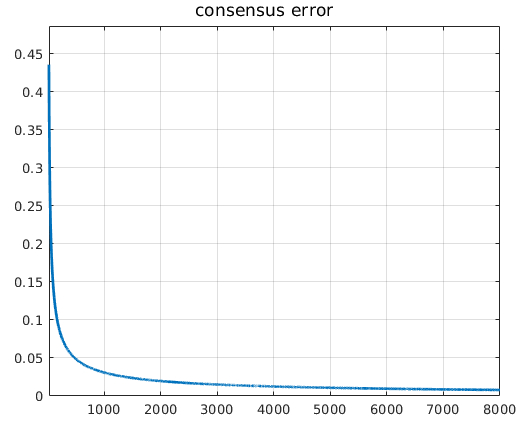
\includegraphics[scale=.45]{images/single_consensus.jpg}
\label{fig: consensus plot}
\end{figure}
\newpage
For sake of clarity, we reported a single consensus error plot.


\newpage
\section{Appendix}
\subsection{Code}
We decided not to add the code to this paper; it can be found on github at this repository: \href{https://github.com/gnoccoalpesto/dcs22}{github.com/gnoccoalpesto/dcs22}

\bibliographystyle{plain}
\bibliography{references}

\end{document}





